\documentclass[journal]{vgtc}                % final (journal style)
%\documentclass[review,journal]{vgtc}         % review (journal style)
%\documentclass[widereview]{vgtc}             % wide-spaced review
%\documentclass[preprint,journal]{vgtc}       % preprint (journal style)

%% Uncomment one of the lines above depending on where your paper is
%% in the conference process. ``review'' and ``widereview'' are for review
%% submission, ``preprint'' is for pre-publication, and the final version
%% doesn't use a specific qualifier.

%% Please use one of the ``review'' options in combination with the
%% assigned online id (see below) ONLY if your paper uses a double blind
%% review process. Some conferences, like IEEE Vis and InfoVis, have NOT
%% in the past.

%% Please note that the use of figures other than the optional teaser is not permitted on the first page
%% of the journal version.  Figures should begin on the second page and be
%% in CMYK or Grey scale format, otherwise, colour shifting may occur
%% during the printing process.  Papers submitted with figures other than the optional teaser on the
%% first page will be refused. Also, the teaser figure should only have the
%% width of the abstract as the template enforces it.

%% These few lines make a distinction between latex and pdflatex calls and they
%% bring in essential packages for graphics and font handling.
%% Note that due to the \DeclareGraphicsExtensions{} call it is no longer necessary
%% to provide the the path and extension of a graphics file:
%% 
\includegraphics{diamondrule} is completely sufficient.
%%
\ifpdf%                                % if we use pdflatex
  \pdfoutput=1\relax                   % create PDFs from pdfLaTeX
  \pdfcompresslevel=9                  % PDF Compression
  \pdfoptionpdfminorversion=7          % create PDF 1.7
  \ExecuteOptions{pdftex}
  \usepackage{graphicx}                % allow us to embed graphics files
  \DeclareGraphicsExtensions{.pdf,.png,.jpg,.jpeg} % for pdflatex we expect .pdf, .png, or .jpg files
\else%                                 % else we use pure latex
  \ExecuteOptions{dvips}
  \usepackage{graphicx}                % allow us to embed graphics files
  \DeclareGraphicsExtensions{.eps}     % for pure latex we expect eps files
\fi%

%% it is recomended to use ``\autoref{sec:bla}'' instead of ``Fig.~\ref{sec:bla}''
\graphicspath{{figures/}{pictures/}{images/}{./}} % where to search for the images

\usepackage{microtype}                 % use micro-typography (slightly more compact, better to read)
\PassOptionsToPackage{warn}{textcomp}  % to address font issues with \textrightarrow
\usepackage{textcomp}                  % use better special symbols
\usepackage{mathptmx}                  % use matching math font
\usepackage{times}                     % we use Times as the main font
\renewcommand*\ttdefault{txtt}         % a nicer typewriter font
\usepackage{cite}                      % needed to automatically sort the references
\usepackage{tabu}                      % only used for the table example
\usepackage{booktabs}                  % only used for the table example
\usepackage{multirow}
%% We encourage the use of mathptmx for consistent usage of times font
%% throughout the proceedings. However, if you encounter conflicts
%% with other math-related packages, you may want to disable it.

%% In preprint mode you may define your own headline.
%\preprinttext{To appear in IEEE Transactions on Visualization and Computer Graphics.}

%% If you are submitting a paper to a conference for review with a double
%% blind reviewing process, please replace the value ``0'' below with your
%% OnlineID. Otherwise, you may safely leave it at ``0''.
\onlineid{0}

%% declare the category of your paper, only shown in review mode
\vgtccategory{Research}
%% please declare the paper type of your paper to help reviewers, only shown in review mode
%% choices:
%% * algorithm/technique
%% * application/design study
%% * evaluation
%% * system
%% * theory/model
\vgtcpapertype{please specify}

%% Paper title.
\title{Crowd-powered Semantic Ineraction for Text Analytics}

%% This is how authors are specified in the journal style

%% indicate IEEE Member or Student Member in form indicated below
\author{Yali Bian, Tianyi Li, Ji Wang, Kurt Luther, Chris North}
\authorfooter{
%% insert punctuation at end of each item
\item
 Yali Bian, Kurt Luther, Chris North are with Virginia Tech. E-mail: [yali, north]@vt.eud.
}

%other entries to be set up for journal
\shortauthortitle{Biv \MakeLowercase{\textit{et al.}}: Global Illumination for Fun and Profit}
%\shortauthortitle{Firstauthor \MakeLowercase{\textit{et al.}}: Paper Title}

%% Abstract section.
\abstract{
Visual analytics could help users explore and gain insight from dataset through interactive visualization and underlying analytics models.
However, making sense of large text dataset is still challenging in many domains.
For example, an intelligence analyst might need to find a coordinated terrorist assault in three US cities from one hundred of documents in a limited time.
Existing visual analytics techniques only assist with low-level tasks, such as finding related documents based on shared entities, which still require significant effort on the part of users.

To support the sensemaking process in visual analytics, we present the concept of crowd-powered semantic interaction, where semantic interactions can be used assign micro-tasks to crowds.
This model could help users to steer crowd-workers to carry out sensemaking tasks implicitly even they are novice on crowdsourcing.
The completed output could be used to update the visualization appropriately that foster the related foraging and synthesis parts for users.
To demonstrate this model, we introduce CrowdSPIRE, a visual text analytics prototype that converts user interactions on documents into micro-tasks called "Connect the Dots".
For example, the user drags two texts together, which triggers the assignment of certain sensemaking tasks to crowdworkers automatically,  in parallel with the expert’s own investigation.
When the tasks finished, outputs could be used to update current visualization appropriately without distracting user's attention from the current thinking.
}

%% Keywords that describe your work. Will show as 'Index Terms' in journal
%% please capitalize first letter and insert punctuation after last keyword
\keywords{Visual analytics, Semantic Interaction, Crowdsourcing, Sensemaking, Crowd-powered Interface. }

\CCScatlist{ % not used in journal version
 \CCScat{K.6.1}{Management of Computing and Information Systems}%
{Project and People Management}{Life Cycle};
 \CCScat{K.7.m}{The Computing Profession}{Miscellaneous}{Ethics}
}

%% Uncomment below to include a teaser figure.
\teaser{
  \centering
  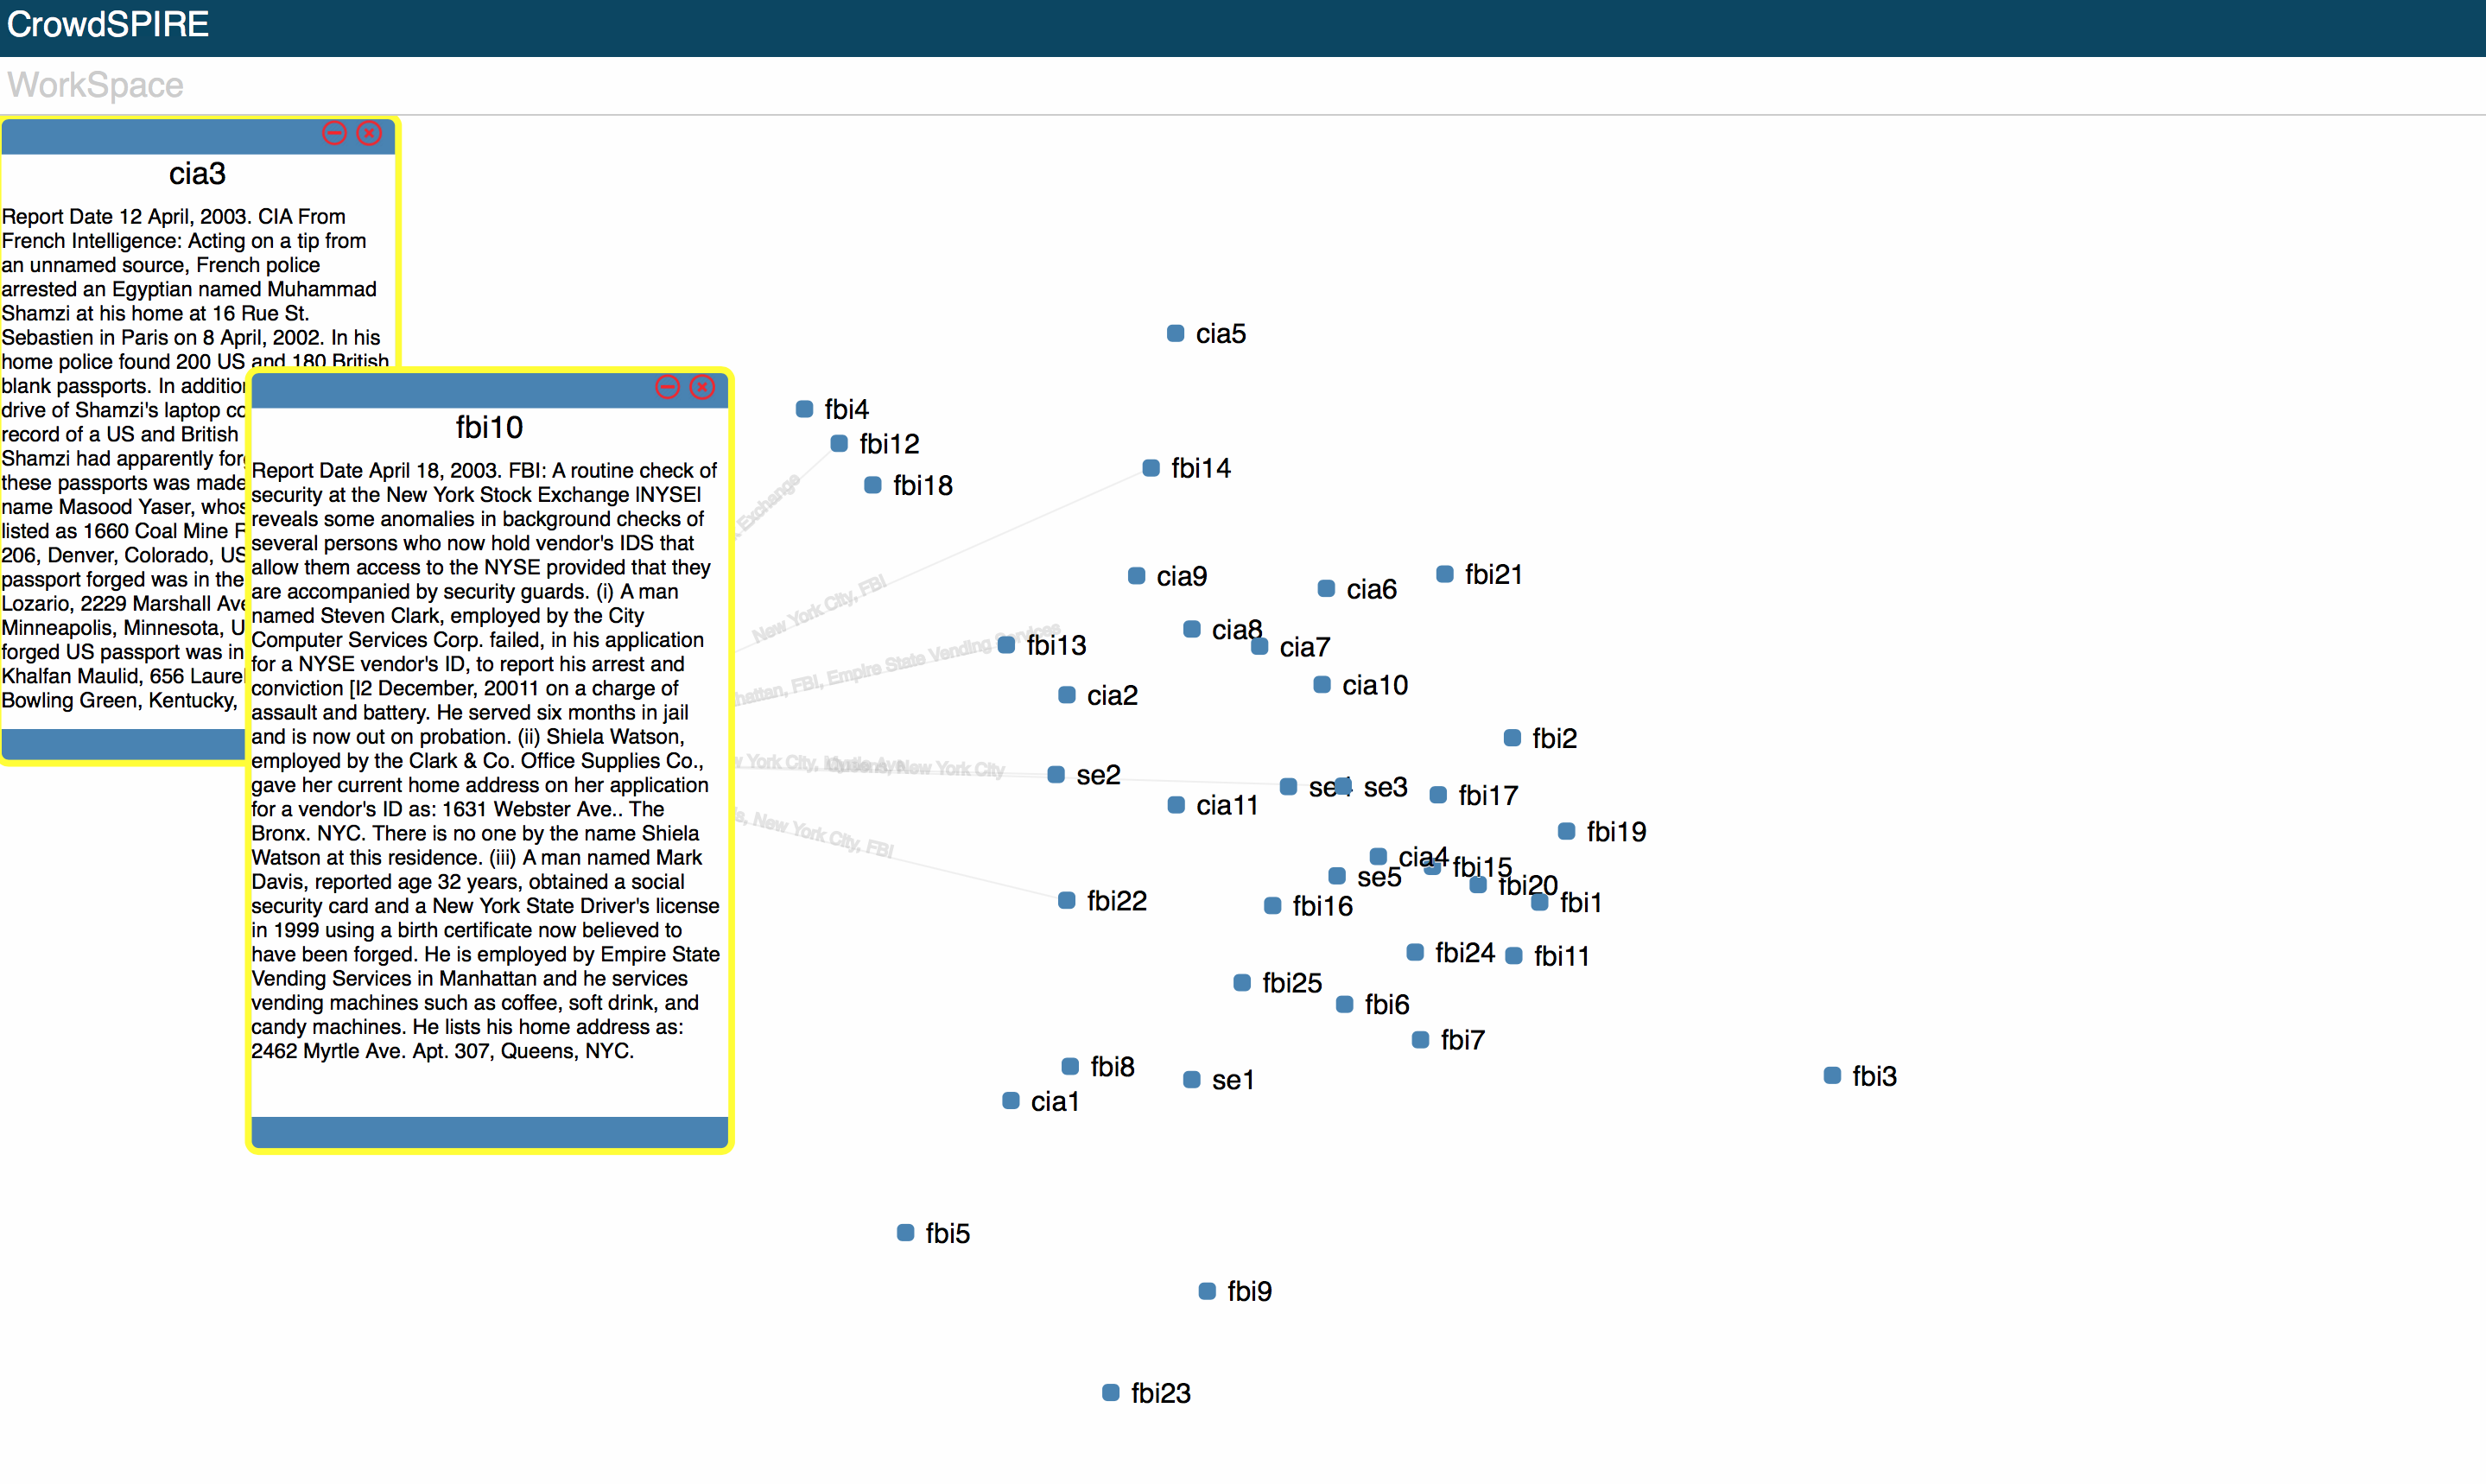
\includegraphics[width=\linewidth]{Overview}
  \caption{Crowd-powered Senmantic Interaction for Text Analytics}
	\label{fig:Overview}
}

%% Uncomment below to disable the manuscript note
%\renewcommand{\manuscriptnotetxt}{}

%% Copyright space is enabled by default as required by guidelines.
%% It is disabled by the 'review' option or via the following command:
% \nocopyrightspace
\vgtcinsertpkg

%%%%%%%%%%%%%%%%%%%%%%%%%%%%%%%%%%%%%%%%%%%%%%%%%%%%%%%%%%%%%%%%
%%%%%%%%%%%%%%%%%%%%%% START OF THE PAPER %%%%%%%%%%%%%%%%%%%%%%
%%%%%%%%%%%%%%%%%%%%%%%%%%%%%%%%%%%%%%%%%%%%%%%%%%%%%%%%%%%%%%%%%

\begin{document}

%%%%%%%%%%%%%%%%%%%%%%%%%%%%%%%%%%%%%%%%%%%%%
%	Introduction
%%%%%%%%%%%%%%%%%%%%%%%%%%%%%%%%%%%%%%%%%%%%%
\firstsection{Introduction}
\maketitle
%% \section{Introduction}
Sensemaking large amount of unstructured text is urgently needed but challenging today. If we can find ways to make sense of this big data, the possibilities for learning more about ourselves and how to improve the world we live in are almost boundless. For example, detecting and preventing a terrorist attack based on intelligence reports. Responding to the challenging, there emerged the field of visual analytics[illuminate the path] that combines the powerful approaches--information visualization and data mining--to create a new class of sensemaking tools enabling new kinds of exploration and insights. (Exemple)

However, it remains time-consuming and onerous, and existing support tools still have a long way to go. Machine learning techniques could help find clusters and summarize documents efficiently, but currently, they cannot generate questions, hypotheses, or conclusions based on data that are more subtle than what an algorithm has been programmed to recognize. What's more, visualization tools amplify the cognitive abilities of their users, but many users could only access to low-level information on documents, which requiring significant effort on the part of users to get the deep insight of data with all kinds of external knowledge. For example, analysts cannot find the relationship between AMTRAK \#19 with a terrist attack if they don't consult the AMTRAK schedules on the Internet to see that Train \#19 is in fact called "The Crescent."


% Corresponding model updates are performed to steer the model based on the user’s reasoning.
% Why Crowdsoucing, why crowdsoucing hard to use
Crowdsourcing presents new opportunities to deal with this issue by augmenting the cognitive work of individual analysts, providing more insightful analysis than automated approaches and scaling better than traditional work. Crowdsourcing was originally used for simple, independent tasks that leverage innate human abilities like transcribing text, identifying images, and categorizing or labeling items[]. Recently, researchers have begun to investigate how crowdsourcing can be applied to complex sensemaking tasks, like creating a taxonomy of items or performing a bottom-up analysis of a large corpus of qualitative data. These efforts show promise for how crowds might assist an individual analyst with a difficult sensemaking problem.

Though crowdsourcing is a powerful method to enhance users sensemaking process, the integration of crowdsourcing into visual analytics could be tough work. Analysts who are non-expert in crowdsourcing might have a hard time to design and assign tasks to crowds. Even they are experts on human computation; they still have to put their time and energy in designing appropriate HITs and putting it to a crowdsourcing platform, which will distract analysts from their current investigation. [More details?]

% Steer crowdsourcing implicitly.
Semantic interaction has been approved to a be a good way to help users focus on their cognition of interesting elements on visualization, at the same time steering underlying models implicitly. Through basic interactions like dragging documents together, highlight important sentences, analysts could steer computational analytical models implicitly, instead of mastering the model first and changing the low-level input parameters of algorithms directly. Semantic interaction provides a bridge between analysts who are non-expert on machine learning algorithms and underlying models.

With semantic interaction, an expert analyst could guide the machine learning algorithms by directly manipulating the visualization layout. Our vision is that the expert interactions will also guide crowdsourcing micro-tasks to do more sensemaking works that machine learning algorithms not good at. We propose the crowd-powered semantic interaction model by coupling visual analytics with crowdsourcing through semantic interaction, and therefore, coupling analysts not only with the ability to parse huge quantities of documents but also the power to make sense of complex tasks effectively.

Designing visual analytics systems with crowdsourcing involves new challenges that we should take into consideration. Visual analytics system should map interactions to appropriate relevant sensemaking-tasks semantically. For example, it is not a good idea to map interaction of dragging two documents aways from each other to micro-tasks that find their similarities. Also, coordinating and aggregating different kinds of tasks to effectively contribute to sensemaking visual feedback is another problem. Since different sub-tasks could have different granularity, information context, correctness, and efficiency.

To address such challenges, we present the crowd-powered semantic interactions to support the combination of visual analytics with human computations. Our key contributions in this paper are as follows:

(1) We propose the crowd-powered semantic interaction model that improve users' sensemaking process through crowdsourcing and formalize this model in the form of an updated visualization pipeline enhanced with crowdsourcing.

(2) We formalize the mapping from interaction to micro-tasks as sensemaking allocation strategies based on the user’s reasoning.

(3) We classify current existing sensemaking crowdsourcing tasks for text analytics based on their granularity and efficiency and explore the solutions to integrate them into real-time visual analytics system.

(4) To demonstrate crowd-powered semantic interaction, we present CrowdSPIRE, a visual analytics prototype based on ForceSPIRE. We present a usage scenario to demonstrate how crowd-powered semantic interactions to be used to help users' complex sensemaking tasks.


\begin{table*}[t]
  \caption{Sensemaking context in each Semantic Interction}
  \label{tab:context}
  \centering
  \begin{tabular}{| m{2cm} | m{6cm} | m{4cm} | m{4cm} |}
  \hline
   \multirow{2}{2cm}{Semantic Interaction} & \multirow{2}{6cm}{Associate Analytic Reasoning} & \multicolumn{2}{c|}{Crowdsourced Subtasks} \\ \cline{3-4} & & Foraging Task & Synthesis Task\\ \hline

Document Movement  &  Similarity/Dissimilarity \newline Create spatial construct (e.g. cluster, timeline, list, etc.) \newline Test hypothesis, see how document “fits” in region &  & Rearrange the spatial workspace to reflect the user’s organizational schema.\\ \hline

Text Highlighting & Mark importance of phrase (collection of entities) \newline Augment visual appearance of document for reference  & Retrieves documents matching the highlighted text from dataset & Find related entities and rearrange the document layout based on highlighted text \\ \hline

Pinning Document & Give semantic meaning to space/layout &  & Rearrange the spatial workspace to reflect the user’s organizational schema.\\ \hline

Annotation, “Sticky Note” & Put semantic information in workspace, within document context & Retrieve documents matching the annotation & Layout current documents on workspace based on annotations, find more links between this document based on the annotation\\ \hline

Open document & Change ease of visually referencing information (e.g., full detail = more important = easy to reference) & Retrieves more documents related to this document & Find more relationships between this document and other documents on current workspace. Re-layout the neighbors of selected document \\ \hline

Minimize document & Change ease of visually referencing information (e.g., full detail = more important = easy to reference) & Retrieves more documents related to this document & Find more relationships between this document and other documents on current workspace. Re-layout the neighbors of selected document \\ \hline

Search Terms & Expressive search for entity & Retrieve more documents matching searching terms & Find related terms have the meaning on current context, Re-layout documents on current workspace based on searching terms \\ \hline


Overlapping documents
& Expressive search for entity & Retrieve more documents that connected with those two documents & Find relationships between overlapped documents and compare their contents, Re-layout documents on current workspace based on the overlapped documents locations\\ \hline
\end{tabular}
\end{table*}

%%%%%%%%%%%%%%%%%%%%%%%%%%%%%%%%%%%%%%%%%%%%%
%	Related Work
%%%%%%%%%%%%%%%%%%%%%%%%%%%%%%%%%%%%%%%%%%%%%
\section{Related Work}
The crowd-powered semantic interaction model involves techniques from three part: visual analytics with semantic interaction, human computation, and sense making model to help combine this two techniques together.

\subsection{Semantic Interaction for Visual Analytics}
% What is semantic interaction
Semantic interaction (Figure 3) was designed to enable analysts to steer computational analytical models in a usable way [8,15,17,23].
Semantic interaction shields the analysts from the low-level input parameters of the algorithms, and instead enables analysts to interact directly with the high-level outputs of the models which is where their cognition is focused.
These high-level interactions are then recast into low-level inputs, through machine learning algorithms that attempt to recognize the reasoning process.
For example, in text analytics, analysts can interact using their normal sensemaking actions such as reading, organizing documents spatially, highlighting important sections, conducting searches, annotating in the margins, etc. In the StartSPIRE prototype, these actions are interpreted by the underlying algorithms and applied to support the analyst by automatically finding and organizing additional information relavant to the analysts' thought process, integrating this visual feedback directly into the analyst's visual spatial workspace.
In our studies, we have found that this method successfully recognized analysts’ reasoning processes and relieved users from the need to organize many supporting documents or read many irrelevant documents [16].

We now recognize the opportunity to apply semantic interaction techniques to enable analysts to not only direct computational algorithms, but to also direct a large force of crowdworkers.
Also, since semantic interaction recognizes opportunities for supporting subtasks and relevant information, it could also be used to support the process of generating dynamic context slices for crowdworkers’ subtasks.

\subsection{Sensemaking}
Two parts of sensemaking phrases: foraging and synthesis.

\subsection{Crowdsourced synthesis and sensemaking, Crowd-powered interface}
Intro to crowdsourcing, then two part intro to how combine crowdsourced synthesis, and How about use crowdsourcing to Visual Analytics.
\subsubsection{Crowdsourced synthesis}
Researchers have explored the value of using Figure 1: The sensemaking loop for crowdsourcing, either alone or combined with intelligence analysts described by [32]. automated approaches, to synthesize information with diverse or unknown schemas. One fruitful approach has been to blend crowdsourcing with ML algorithms. Partial clustering [19,40] and crowd kernel [35] are two such examples, but their application domain limited to imagery, and they focus on low context merges between pairs or triplets of items.

Other crowdsourcing research explores higher-context clustering. Cascade [12] produces crowdsourced taxonomies of hierarchical data sets by letting workers generate, and later select, multiple categories per item. Frenzy [11] is a web-based collaborative session organizer that elicits paper metadata by letting crowdworkers group papers into sessions using a synchronous clustering tool. We draw design inspiration from these projects, particularly the notion of integrating microtasks into a more collaborative, unstructured interface embodied in Frenzy and other forms of crowdware [41]. Our prior work builds on this research by evaluating these clustering-style interfaces compared to other interfaces and workflows.

Researchers have also studied how much context to provide crowdworkers during clustering tasks. Willet et al. [39] developed color clustering with representative sampling for reducing redundancy and capturing provenance during crowdsourced data analysis, comparing this to a pairwise “distributed clustering” approach. Andre et al. [2] compared automated clustering via TF-IDF [34], Cascade [12], and crowdsourced partial clustering adapted from Gomes et al. [19], finding that all three methods could outperform collocated experts in developing conference paper sessions. Andre et al. [1] experimented with giving crowdworkers different amounts of context prior to clustering Wikipedia barnstars. Our prior work expands on these studies by investigating a higher upper bound for context, its interaction with task structure, and synthesis across multiple documents.

Our proposed research builds on these earlier projects in significant ways. First, and most importantly, our unit of analysis is the entire sensemaking loop and ways that an individual analyst can be supported in real time by crowds or computation. We seek to augment the capabilities of these analysts, regardless of their expertise, allowing them to work faster accomplish more than they could unaided. To this end, all of our studies focus on how crowds or computation ultimately contribute to the performance of this individual. This approach is a significant departure from the majority of prior work that emphasizes unsupervised crowdsourced or computational techniques aimed at matching the performance of a motivated individual for a specific task or situation. Second, unlike most crowdsourced sensemaking projects that focus on either images or text, we investigate both domains to identify generalizable patterns and distill cross-domain design principles. Third, while prior work (including our own) establishes the importance of giving crowd workers the right amount of context, we extend this work by introducing the concept of dynamic context slices, which uses one of several methods to give each worker an amount of context customized to his or her unique task.

\subsubsection{Real-time crowdsoucing and Crowd-powered interface, human in a loop}
Real-time crowdsourcing systems have been developed to assist individuals with sensemaking tasks [5,6,26,27]. For example, VizWiz [6] is a mobile app that lets blind users capture images that sighted crowd workers can describe for them, and Chorus [27] provides a chat interface for crowd workers to help users with online search tasks like finding a nearby restaurant. We take inspiration from these systems, especially their mechanisms for recruiting and aggregating crowd work in real time, and extend them to complex sensemaking tasks where crowds are directed by mechanisms other than explicit user requests.

In this paper, we focus on the crowdsourcing of such plans as a case study of constraint-based human computation tasks and introduce a collaborative planning system called Mobi that illustrates a novel crowdware paradigm. Mobi presents a single inter- face that enables crowd participants to view the current solution context and make appropriate contributions based on current needs.


%%%%%%%%%%%%%%%%%%%%%%%%%%%%%%%%%%%%%%%%%%%%%
%	Crowd-Powered Semantic Interaction
%%%%%%%%%%%%%%%%%%%%%%%%%%%%%%%%%%%%%%%%%%%%%
\section{Crowd-powered Semantic Interactions}

% \begin{figure}[tb]
\begin{figure*}
 \centering % avoid the use of \begin{center}...\end{center} and use \centering instead (more compact)
%  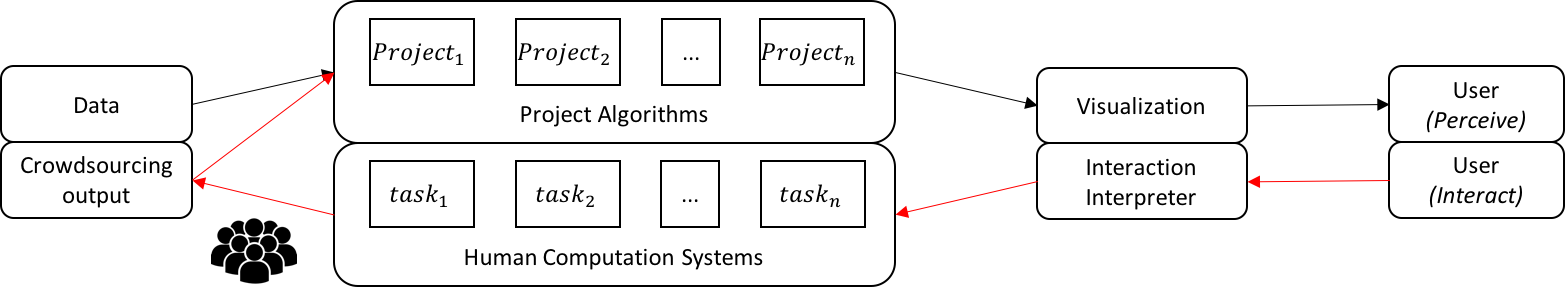
\includegraphics[width=\columnwidth]{Pipeline}
  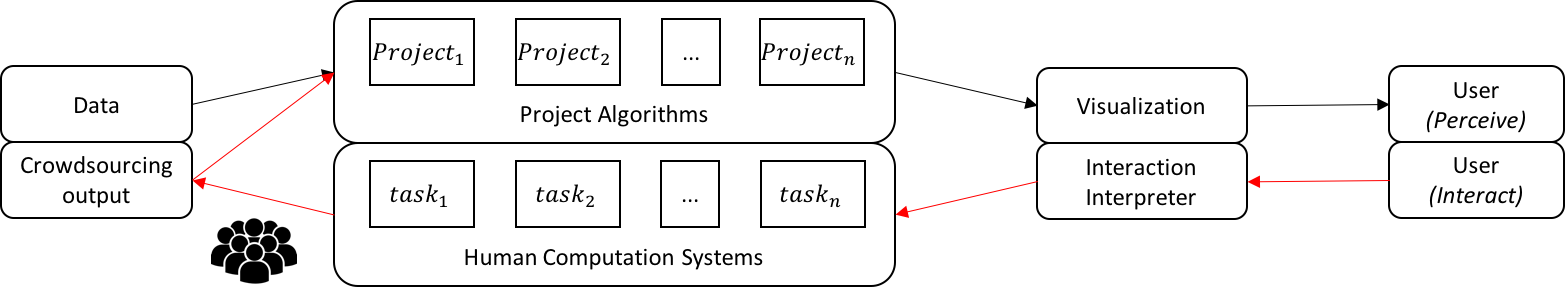
\includegraphics[width=\textwidth]{Pipeline}
 \caption{crowdsourcing based semantic interaction visualization pipeline.
 Once the user perceives the visualization, they can choose to interact in it.
 This interaction feedback is interpreted as requests to the human computation system, which could assign several micro-tasks to crowds.
 The project algorithms could update visualization based on crowdsourcing outputs through their types, along with original data.
	 }
 \label{fig:pipeline}
\end{figure*}


% Main idea and examples to explain the idea.
To help boosting the sensemaking phrase of analytics, we propose the novel idea of combining visual analytics with crowdsourcing.
However, to combine this two fields appropriately and make full use the advantages from both field, we extension the idea of semantic interaction, that help expert analysts guide the machine learning algorithms by directly manipulating the layout, into the crowdsoucring field: that use semantic interactions to guide crowdworkers' subtask automatically and update the visual interface appropriately when tasks finished.
Ultimately, this system design will be two major step towards developing powerful software tools to augment human intelligence and sensemaking:

(1) Generate and design tasks automatically based on semantic interaction: We will begin by generating a list of potential subtasks to be modularized and decomposed from the sensemaking process,the sensemaking process be most effectively divided between individuals, crowds, andHow can the sensemaking process be most effectively divided between individuals, crowds, and computing? What are the finest granularities of tasks that can be effectively aggregated to contribute to sensemaking? How much information context is necessary for an individual to contribute meaningfully to a collaborative sensemaking effort? computing? task allocation strategies, perform complex sensemaking using crowdsourcing while minimizing bottlenecks and redundancies?
We envision an expert analyst working in a sensemaking environment that observes and dynamically responds to her reasoning process.
As the expert begins working, certain sensemaking subtasks, e.g. foraging and synthesizing, can be spun off from the expert and performed by crowdworkers, or handled automatically, in parallel with the expert’s own investigation.
The spin-off process may occur explicitly, initiated by the expert herself as a kind of crowd delegation, or implicitly, by the system analyzing her activities and generating predictions of promising lines of inquiry.
The crowd might even direct itself, drawing on human intuition and hunches.

(2) Integrate completed task results into the visual interface in the appropriate context.
As crowdworkers enter and leave their work environments, context slices allow them to complete tasks or pass on their works-in-progress to the next crowd. The completed results are integrated into the expert’s workspace in the appropriate context.
prior work comparing tournament (parallel) versus linear (serial) crowdsourcing workflows for synthesizing diverse information sources provides a strong foundation
As crowdworkers enter and leave their work environments, context slices allow them to complete tasks or pass on their works-in-progress to the next crowd.
The completed results are integrated into the expert’s workspace in the appropriate context.
Consequently, the expert is able to solve the sensemaking problem much more quickly, with lower total effort, than she could ordinarily.

% Example on Crowd-powered Semantic Interaction
As an example, an expert working in intelligence analysis may be investigating three different individuals suspected of being involved in a terrorist plot.
He and his colleagues have collected a large corpus of potentially relevant documents including police reports, depositions, surveillance footage, and other materials.
The expert launches our software on a computer with a large display and begins sifting through and grouping related documents.
He puts three documents about Suspect 1 together to form a cluster, and makes another cluster with two documents related to Suspect 2.
He begins work on Suspect 3.
Meanwhile, the software begins seeking potential connections between suspects using both computational and crowd-based techniques.
A data mining algorithm identifies simple connections between the suspects based on overlapping metadata, such as the fact that Suspects 1 and 2 live in the same state, but this connection is unimportant to the analyst.
The software also recruits crowdworkers to examine the clusters and suggest potentially relevant connections between the two suspects and five documents.
Buried deep in the documents is a surprising connection: both suspects own multiple luxury cars.
The system highlights this crowd-identified relationship for the expert, who notices the update, and begins formulating a hypothesis about the two suspects working together and receiving a large payment.


%%%%%%%%%%%%%%%%%%%%%%%%%%%%%%%%%%%%%%%%%%%%%
%	Updated Visualization Pipeline
\subsection{Updated Visualization Pipeline}


We present an updated visualization pipeline to reflect crowd-powered semantic interaction model.
The initial visualization is constructed by taking the data, or a working set of the data as determined by a relevance model, and passing it through a display layout model.
The user then perceives the visualization and has the option of interacting with the data within the spatial metaphor.
All interactions are interpreted and directed to the appropriate tasks based on task allocation strategy.
For each interaction, the task allocation strategy could assign several sensemaking sub-tasks (foraging and synthesizing) based on current contexts(elements showed on screen) to crowds. Some sub-tasks could also be combined to support other complex sub-tasks.
After several times of recursion, the completed tasks' output combined with original data could be mapped to visualization based on appropriate current contents. Only related information could be used to update the visualization, other information from crowd might disturb the human in a loop. This pipeline currently assumes a single layout model used on our visualization system.

Possible extensions of this pipeline include multiple automatic computation models for the data (e.g. the user believes the data should be arranged in a different manner than what the user believes should be displayed), on interaction interpreter to help find and define more needed crowd tasks.
Not all semantic interactions will necessarily start and assign the crowd task since original interactions could have already finished the tasks.
For examples to illustrate this point.
Highlighting a phrase in a document typically indicates its importance, while minimizing a document when space is not constricted typically indicates the unimportance of its contents.
Moving points around the display would naturally update the display layout, but would not necessarily fetch new data points for the workspace.

Tasks outputs could be stored so that users can make use of external knowledge in the future, instead of create a new tasks.




%%%%%%%%%%%%%%%%%%%%%%%%%%%%%%%%%%%%%%%%%%%%%
% Task allocation strategy
\subsection{Task allocation strategy}

% Define sensemaking tasks. on two phrase.
Since semantic interactions right now are mainly on spatilation. We, design sensemaking tasks main on their relationships.
For each interaction, semantic interaction could help us understand each of their reasoning, which we could define several sensemaking tasks.
And each sensemaking tasks could be modularized and decomposed, to several sub-tasks so that crowdsourcing could be used to perform them.
Different phrase have different contexts,
Current senmaking tasks. For example, when searching new words, at the foraging loop, the context is the whole dataset. If highlight a setence on an opened document, the main context is current documents on the screen.

create multiple alternative competing hypotheses based on the given data
find additional relevant information that supports the created hypotheses.
dual search, occurs between these two loops in which analysts must simultaneously create multiple alternative competing hypotheses based on the given data and, at the same time, find additional relevant information that supports the created hypotheses.

Based on different sensemaking tasts and their context, we could design to the task based on task allocation strategy.
For each of those sensemaking task, we could design several kind of sensemaking tasks to get a clear results.
What's more, for each interaction, there is a context, that describe current sensemaking issues.
How the sensemaking tasks identified in that study could be modularized and decomposed, so that either automated techniques, or crowdsourcing, could be used to perform them. The goal of this study is to generate automated or crowd-powered alternatives to individual analysts performing these tasks, towards the goal of augmenting analysts with a suite of support tools. To reach this goal, we will perform a series of experiments to identify the benefits, drawbacks, and tradeoffs of using individuals, automated techniques like data mining, and crowdsourcing for each component of the sensemaking process.

The details of each subtask experimental procedure will vary depending on the details of the subtask alternatives; for example, foraging subtasks imply different participant goals than synthesis subtasks. However, in general, our goal is to devise and compare individual analyst performance and subjective experiences to those of crowdworkers, as well as a state-of-the-art automated approach. Crowdworker tasks and interfaces will be designed to assume minimal worker skill and expertise, to be verified using pre-survey screenings.

We convert the translates the sensemaking tasks into real problems like the distance between documents, which is a unified task purpose to do tasks and update the visual interface.

Spatializations are frequently employed to aid sensemaking (foraging and synthesis) of unstructured text documents [2, 21, 30, 33, 34].
Large, high-resolution displays in particular have been found beneficial in affording a large, flexible workspace that allows users to externalize knowledge and create semantic schemas.

For different interactions, the difference is that we get different contexts, and informations for this task.
Also, each interaction, we could reason this interaction from two kind of sensemaking phrase: based on the associate analytic reasoning, we list the task like this:


Two sensemaking phrase provide different functions, the foraging part is responsible for gathering relevant information based on current user's intention which could be expressed through interactions with the visualization. Even for the foraging crowdsourcing tasks, different interactions, could assign different level of foraging tasks: for example, text highlighting could trigger.


Right now semantic interactions are mainly based on spatiation, so the purpose of sensemaking tasks could also be the layout of statialation.

Users could make sense of dataset in details through interaction like searching.
For example, ForceSPIRE[] provides a list of various forms of semantic interaction, including how each can be used within the analytic process of investigating textual information spatially.
is list is likely incomplete, but serves as a starting point to introduce how semantic interaction can be integrated into a user’s reasoning process.
Each interaction corresponds to reasoning of users within the analytic process.
Corresponding model updates are performed to steer the crowd-tasks assign system.
Based on different resoning of each interaction, that users use when they want to find more details about interested information about certain word, document, compare between two documets, or a cluster of documets.
they want to narrow down the prolem.

** Semantic interaction and their context
For each semantic interaction, they have a object to specifid, which narrow down theire thinks to (Search for relations/in shobox)
When they open document,
As corresponded to past semantic interaction when they INTERPRETING interactions with ASSOCIATED ANALYTICAL REASONING
In interpreting the interaction, the system determines the analytical reasoning associated with the interactions and updates the model accordingly. From previous findings [5], categories of user interaction can be associated with specific forms of analytical reasoning (see Table 4.1). It is essentially the model’s task to determine why, in terms of the data, the interaction occurred, and how that information can be used to augment and adjust the analytic models of the system to help the user’s task. e goal is to calculate, based on the data, what information is consistent with the captured interaction. For instance, we can associate text highlighting with adding importance to the text being highlighted.
Since, each interaction have a reasoning when they do some interaction at specific level visual elemenets on visualization.
Their sensemaking phrase could have a implicit specified context, based on [5].
Right now we list the implicit context as follows:

The context users used for sensemaking are as follows:

With diferent context:

As shown on tabel \autoref{tab:context}, when user drag two document together, this means on the context of whole documets shown on screen(dataset), they think those tow doucments are similar, we should assign crowd that based on those two documents, we need find more related documents,
and why those two documets are

Levels of documents could be mapped to different kinds of crowd tasks.

Why we assign crowd in this a way, because of sensemakings
There are two very important factors that steer the crowd taks assignment part: sensemaking context, associate analytic reasoning.

For the associate analytic part, we could understand why two documents are related.
For the associate analytic part, we could get more knowledge on this sensemaking context.

The crowd could help users find high level concepts from documents,

Using crowdsourcing to help booster the sensemaking process through two part: foraging and synthsis.

Crowd Synthesis: make clusters.

As such crowd-workflows become complex, researchers must identify the level of crowd-supervision needed for optimal output.
Intead of let crowdsourcing design experts to assign tasks to crowds, we use semantic interactions to latently

HIT Design based on Semantic Interactions

For different semantic interactions, we could assign different tasks.
input:  how to use semantic interaction as input to direct the crowd tasks

can create several kinds of micro-tasks for each SI, some quick, some slow  (simulated in this paper with Tianyi data?) \newline
Drags two docs togethers
1) e.g. when expert drags 2 docs together:

a) find entities that connect the 2 docs (quick)
b) label semantic-level connections between the 2 docs (quick) -> text that can be used
c) find related docs (slow)
i) must compare to every other doc?
ii) or use (a) and (b) to reduce the search set?  context slice?\newline

%%%%%%%%%%%%%%%%%%%%%%%%%%%%%%%%%%%%%%%%%%%%%
% Task allocation strategy
\subsection{Integrate Crowds into Workspace}

synchronous tasks
How to integrating microtasks into a more collaborative, unstructured interface embodied in Frenzy and other forms of crowdware
Human computation
Open Document
Search Keywords\newline
Clusters \newline

% integrated into the expert’s workspace
To integrate the crowds into visual analytics, we need to merge all the sub tasks into formated and combine the modularized subtasks in to a comprehensive sensemaking loop. To doing that, we should general the combination into two things: tasks levels (sub-tasks), and  tasks time complexity.

considering how to recombine the modularized subtasks identified in the previous studies into a comprehensive, revised sensemaking loop, and to implement a software prototype based on this revised process.
This effort implies a modification of the traditional sensemaking loop that accounts for the modularized components developed in Study 2.
We plan a series of experiments leading to the design of effective workflows and task allocation strategies that allow individuals, crowds, and computation to synergistically perform complex sensemaking tasks, while minimizing bottlenecks and redundancies.


\subsubsection{Crowds tasks in different levels}

Crowds sensemaking tasks, based on different phrase, could be divided into two functions: foraging phrase: find more related documents on datasets.  Find documents not based on whether they are entities related but also semantically related.

synthesis phrase: synthesize information with diverse or unknown schemas:

For the first phrase, we could translate the tasks output into distances or orders that which one close to each other.

For synthesis sub-tasks: we could find their schemas on three different levels based on different interactions.

Other level of relationships: compare the similarity between two overlapped documents, based on their contents, if has connections between each other, based on shared entities. or has same high level concepts. For this kinds of tasks, we needs store their outputs in three levels:
entity links
documents similariitys.
clusters.

Entity level tasks
\begin{table}[tb]
  \caption{Sensemaking tasks in different levels}
  \label{tab:tasks}
  \scriptsize%
	\centering%
\begin{tabular*}{\linewidth}{l@{\extracolsep{\fill}}lll}
  \hline
   Interaction & Task Schemas Level & Task demo\\
  \hline
   Keywords &  \\
  Minimizie document & B \\
  Close document & A, B \\
  Annotation & A \\
  Search & A, B \\
  Highlight & A, B \\
  Overlap documents & A, B, C\\
  Cluster documents & D \\
  \bottomrule
\end{tabular*}
\end{table}

How to tranverse outs puts into workspaces.
For each kind of crowdsourcing tasks, we could integrate the results into workspaces.

Also, micro-task are not independent, micro-tasks could designed for each other automatically, for example, linked dots could be used as inputs or contraints for another subtasks.

Right now, crowdsourcing tasks for sensemaking could be classified into three levels: entities, documents (VizWiz: Nearly Real-time Answers to Visual Questions.
find contents on documents, or edits , Frenzy: Collaborative Data Organization for Creating Conference Sessions.),
clusters (Crowd Synthesis: Extracting Categories and Clusters from Complex Data.,  ). For each kinds of crowdsourcing tasks, each kind of crowdsourcing could build on each other.
Lots of details on

Find entities that connect the 2 docs (quick)
For the entities level, we could be used to used as the input to other two level inputs. Also could used to provides as the inputs for automatic computation models.

For document level, we could find more related documents, or find similarity or dissimilarity between small number of documents (usually less than five documents). Find related documents, or remove unrelated documents. Directly to the documents,

For cluster level tasks, we could map the layout to the workspace directly, as a distance function.

label semantic-level connections between the 2 docs (quick) -> text that can be used
find related docs (slow)

output:  how to use crowd output in response to semantic interaction in the visualization
can use crowd results in visualization (e.g. distance function for Force Directed layout)
can use crowd results in further algorithmic processing (e.g. search)
dynamic output, streaming from crowds

\subsubsection{Crowds tasks in different time complexity}

an individual analyst can be supported in real time by crowds or computation.

Real-time crowdsourcing systems have been developed to assist individuals with sensemaking tasks [5,6,26,27].
We seek to augment the capabilities of these analysts, regardless of their expertise, allowing them to work faster accomplish more than they could unaided.

real time
For synthesis phrase tasks, main on a small number of documents,

For most foraging phrase tasks, since there are lots of documents to compile, automatic models could help to find the most possibly related documents, to let crowds to find. It might still be an time-assuming works(more than five mining):
streaming
batching results

for those crowdsouricng tasks, there are two approaches to maneging latency in crowd-powered interfaces: steaming, batching results.
Even if the crowdsourcing tasks are too slow to fit into the human in the loop (react less than ten seconds, the crowdsourcing could still be store to knowledge base, as an external knowledge for latter use, for example, analyst went to the similar situation, like overlap two document again, instead of assign a new task, the system could get crowdsourcing outputs immediately)


If current context changed, store data for latter use.


%%%%%%%%%%%%%%%%%%%%%%%%%%%%%%%%%%%%%%%%%%%%%
%	CrowdSPIRE
%%%%%%%%%%%%%%%%%%%%%%%%%%%%%%%%%%%%%%%%%%%%%
\section{CrowdSPIRE}
\begin{figure*}
 \centering
  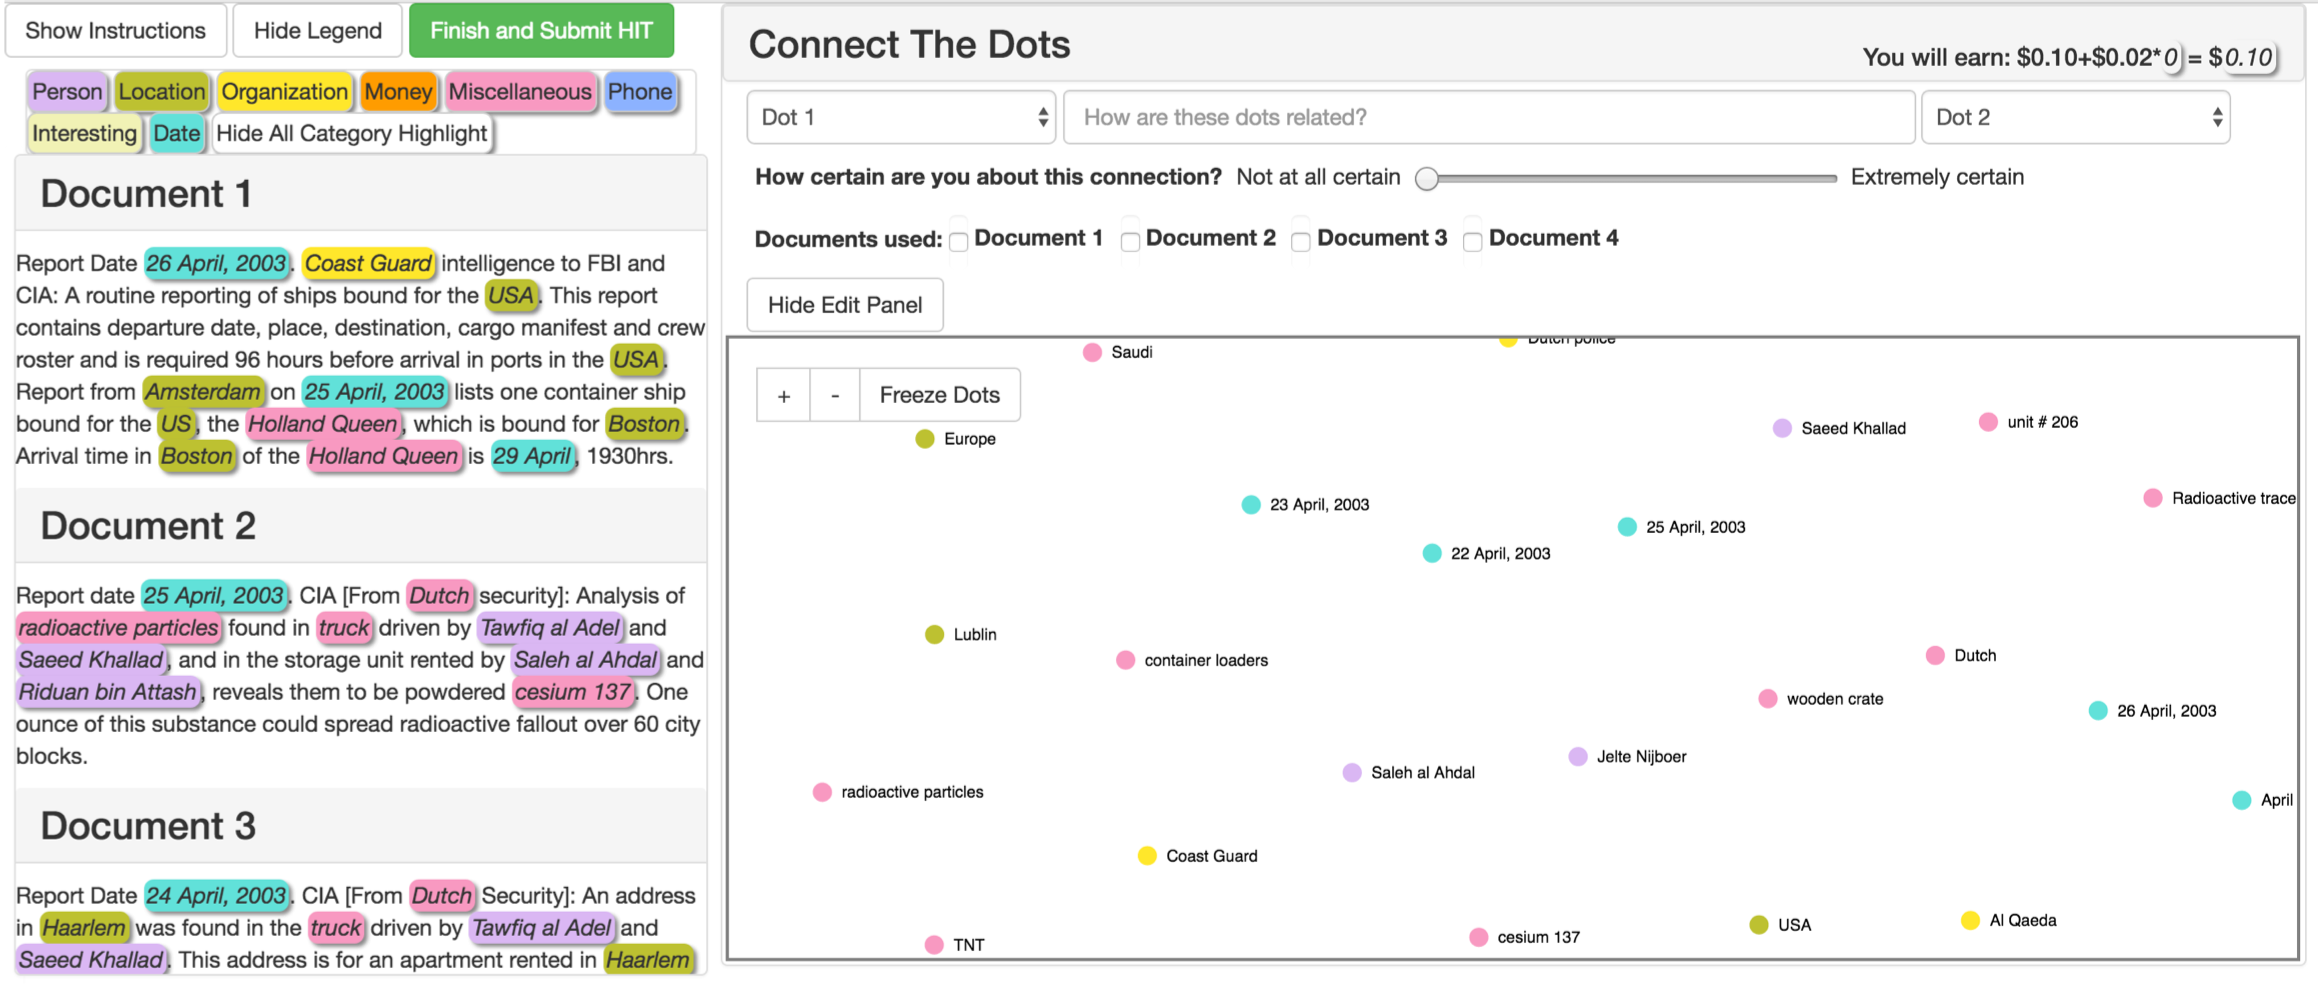
\includegraphics[width=\textwidth]{Hit}
 \caption{The Connect the Dots web application interface}
 \label{fig:hit}
\end{figure*}

说明一下系统是用了机器学习的东西的,为了保证其他交互和StartSPIRE的一致.
CrowdSPIRE (Crowd-powered Spatial Paradigm for Information Retrieval and Exploration) is a visual analytics tool prototype that implements crowd-powered semantic interaction technique: like ForceSPIRE, a semantic interaction visual analytics tool prototype for exploring unstructured text documents.
CrowdSPIRE and ForceSPIRE share a flexible spatial workspace (driven by a modified force-directed layout and several semantic interactions.
However, with different models on the background to help calculate the layouts of documents.
Instead of using machine learning models, CrowdSPIRE use human computation to help calculate the distance between documents and update the layout of workspace.

Right now, CrowdSPIRE integrate the "Connect the dots" tasks, which let crowds labels related entities in documents in a context slice and helps crowd workers with the micro-task of creating and labeling connections between entities extracted from the text.
Through related entities in each document, we could calculate their TF-IDF similarity. When doing overlapping two documents.
This system extends upon previous work to integrate relevance-based retrieval and layout models, provides richer visual encodings, and adds to the semantic interactions leveraged.

StarSPIRE dynamically adjusts how many data points are displayed by using heuristic-based relevance metrics.

Difference from basic pipeline.
% Crowd-sourcing part
% Document overlapping part.

%%%%%%%%%%%%%%%%%%%%%%%%%%%%%%%%%%%%%%%%%%%%%
%	Visual Encoding
\subsection{Visual Encodings}
Within the spatial workspace, document nodes are visually encoded to relate their relevance to the user’s high dimensional understanding of the data [Figure 5].
Node size and saturation are encoded to reflect how closely a document matches the entities the user has deemed important.
Node size and saturation are calculated by summing all of the entity weights in a document, ranking these values, and sorting them into quartiles.
Quartiles were chosen instead of absolute
ranking to optimize the node drawing process, minimizing the number of calculations and changes required with each user interaction.
This was done to promote a quick interaction-feedback loop.
These encodings give the illusion of a third dimension in the workspace where more important documents are in the foreground while less important documents fade into the background.
However, unlike a true three-dimensional layout, document nodes cannot overlap each other, preventing occlusion.
Additionally, StarSPIRE provides visual cues for navigating the workspace.
Node color is used to indicate search term matches.
Instead of showing all links between all documents, StarSPIRE restricts the edges shown to those connected to the selected node.
Entities shared between documents are labelled on the edge, but are restricted to the top four entities, determined by their importance weights.
All nodes are labelled with their document’s titles in order to allow for easier navigation in the space and to allow users to track a specific node’ s movement throughout the space.
Each node’ s outline color is used to denote its read or unread status in order to allow analysts to see which documents they have read and closed.

Within each document, search terms are identified and the text color is changed to allow the terms to stand out for easier identification.
These encodings were identified and/or adjusted through an informal usability requirements analysis of StarSPIRE.

%%%%%%%%%%%%%%%%%%%%%%%%%%%%%%%%%%%%%%%%%%%%%
%	Crowd-powered Document Overlapping
\subsection{Crowd-powered Document Overlapping}
CrowdSPIRE implement all the interactions on ForceSPIRE, users could explore the whole datasets based on document movement, text highlighting, pining document, annotation sticky note, open document, minimize document and overlapping documents. However, to make the system simple and easy to evaluate, we only combine document overlapping interaction with crowdsourcing tasks.

To evaluate the crowd-powered semantic interaction model, we only combined the document overlapping interaction with crowdsourcing tasks.
At first, we have the distance between documents based on algorithms models.

We two or more documents overlapped each other, the semantic interaction will trigger the task allocation stregory design a connect the dots crowdsourcing, based on overlapped documents.

We define D as the set of overlapped documents, for each
To carry out the 'connect the dots' task that help synthesis the overlapped documents:
The task allocation strategy procedure that automatically assign current overlapping interactions to task:\newline
(1) Pick m documents d1, dj from D (i != j), for all the di, dj. \newline
(2) Generate a Hit to MTurk that show m documents:
(2)	Show di, dj to k workers on a visualization view sub-task, which requires workers connect the related entities if they are related. \newline
(3) For each link, the worker should input the certain, and how are these dots related. Document used to make this connection \newline

For example, if three documents d1, and d2 and d3 are overlapped to each other, one of the micro-tasks is on Figure 1: {d1, d2}, {d1, d3} ... will be formed to give tasks to differnet.

based two documents, the connect the dots will publish an Hit on MTurk

%	Integrate 'Connect the Dots' into Workspace
%%%%%%%%%%%%%%%%%%%%%%%%%%%%%%%%%%%%%%%%%%%%%
% Integrate
\subsection{Integrate "Connect the Dots" into Workspace}
To make full use of the 'Connect the Dots' tasks as a real time services, we prototype the task, before the overlapping interactions.
For example, instead of design the hit, after the semantic interaction, we pre-assigned the task, and store outputs to the database, when the overlapping interaction be implements, we retreave this context, as it is.
The related nodes could also be mapped to distances. based on
BAsed on algorithms. Aslo, mapping the distance functions based on related entities.
Pre-store current storage to mimic the real time crowdsourcing.

%%%%%%%%%%%%%%%%%%%%%%%%%%%%%%%%%%%%%%%%%%%%%
% Case Study
%%%%%%%%%%%%%%%%%%%%%%%%%%%%%%%%%%%%%%%%%%%%%

%%%%%%%%%%%%%%%%%%%%%%%%%%%%%%%%%%%%%%%%%%%%%
% Evaluation
%%%%%%%%%%%%%%%%%%%%%%%%%%%%%%%%%%%%%%%%%%%%%
\section{USAGE SCENARIO}


In this section, we will demonstrate how CrowdSPIRE helps an analyst to make sense of complex dataset.
We use The sign of the Crescent dataset[ref] which contains 41 fictional intelligence reports regarding a coordinated terrorist plot in three US cities.
We will evaluate the effectiveness of CrowdSPIRE, we make a comparison of crowd-powered visual analytics (CrowdSPIRE) and algorithm-only based visual analytics (ForceSPIRE).
Also, to test that the crowdsourcing tasks outputs correctness that we compare the layout of documents based on crowdsourcing with the gold standard solution/and the most correct layouts we get when users make sense of documents.
\begin{figure*}
 \centering
  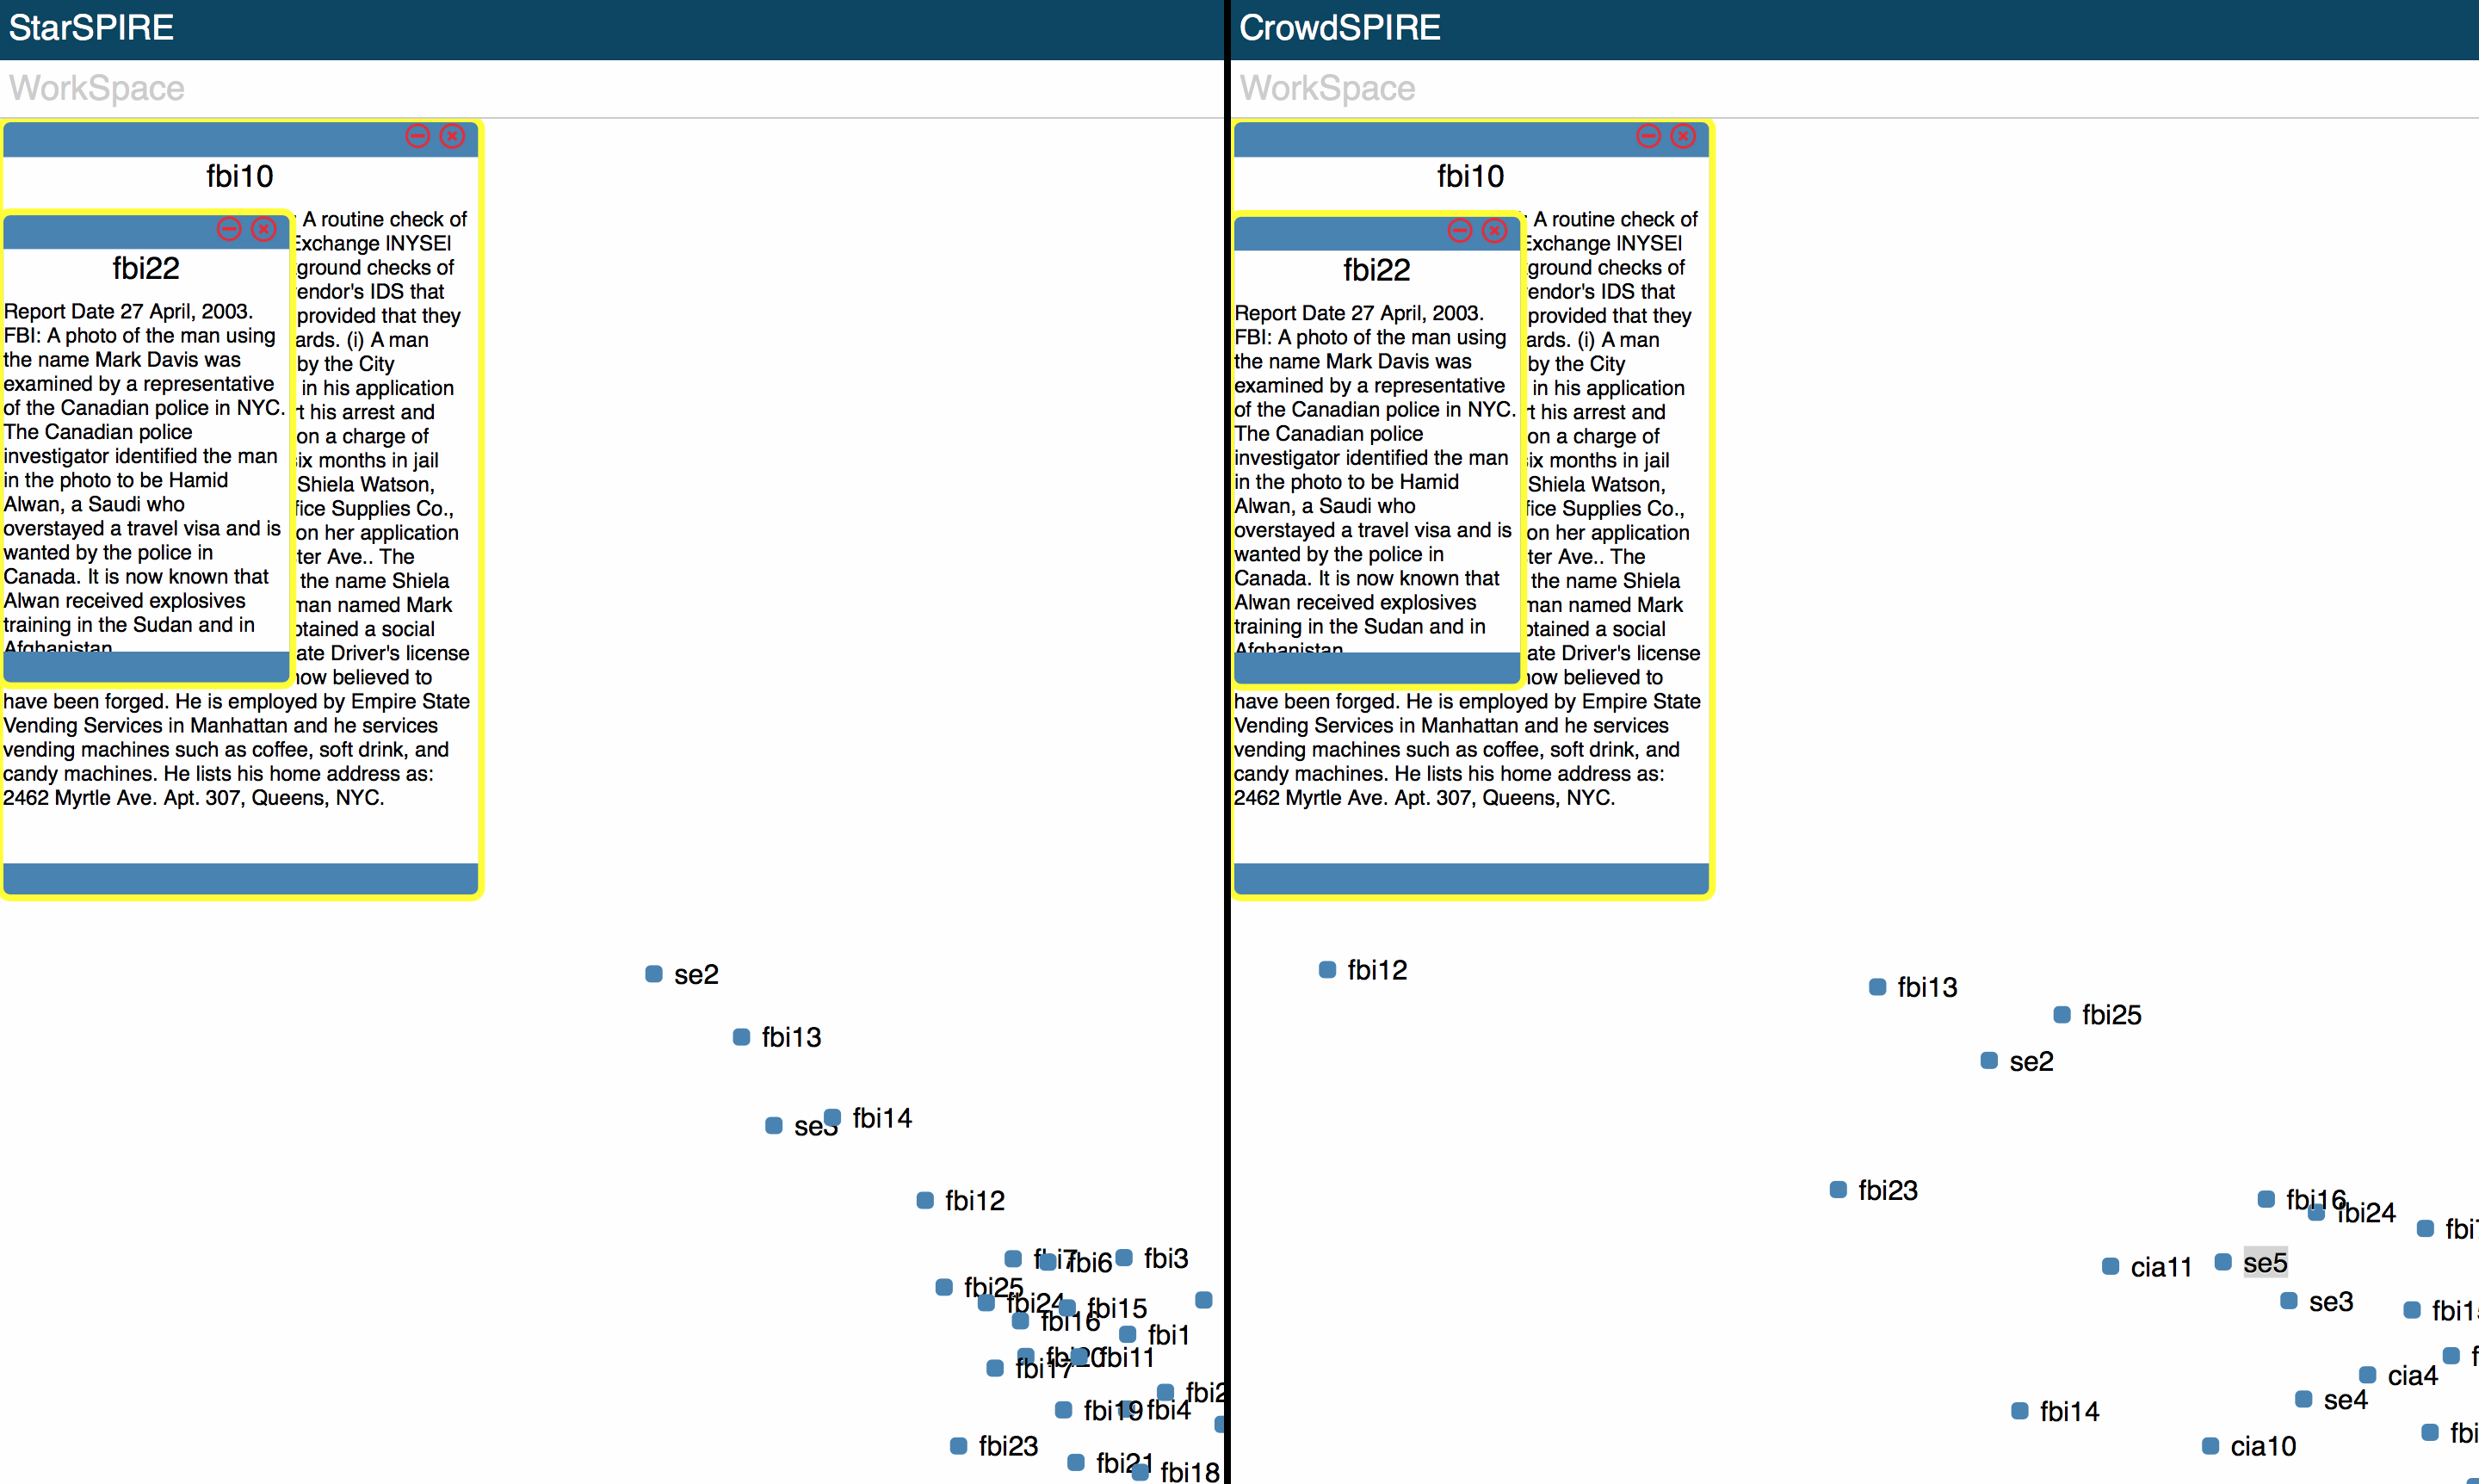
\includegraphics[width=\textwidth]{Case}
 \caption{A process of finding a major threat plot with key steps. (1): Based on A. Ramazi, finding that there are two similar bundles and two cells. (2): One name and two bundles are highlighted when hovering the mouse over B. Dhaliwal. (3): Three names and three bundles are highlighted when exploring F. Goba. (4) Referring to the four connected groups of useful entities for hypothesis generation.}
 \label{fig:case}
\end{figure*}

In this section, we walk through a text analytics scenario to demonstrate the how crowdsourcing supports
Comparison of crowd-enhanced version (CrowdSPIRE) with algorithm-only version(ForceSPIRE).

We prototype a web-version ForceSPIRE at the same version.
The different between ForceSPIRE and CrowdSPIRE is that when overlapping documents together:
ForceSPIRE will trigger the underlying machine learning alorithm to help calculatet the distance between documents.
CrowdSPIRE will trigger the crowd micro-tasks allcation alorithm to assign "Connect the Dots" micro-tasks, and then use the output to calculate the document distance.

So if we let the a user explore the doucments through this two documents, with the same interaction except overlapping documents, they will get similar layout.
Through the layout of overlapping documents interaction, we could analyse current layout that could help user make sense of documents.

For example, if we drag document together, the different layout on two techniques could help use analyse the effectiveness of CrowdSPIRE.

To demonstrate StarSPIRE’s functionality, we used the VAST 2007 Challenge Dataset (“Blue Iguanodon”) [17].
Because StarSPIRE is currently designed to operate on unstructured text documents only, we omitted all images and spreadsheets from the dataset, resulting in approximately 1,500 text files.
Blog entries that were included in the data were converted into text files, one for each blog entry.
Preliminary entity extraction was done on the dataset.
The challenge task is an open-ended sensemaking task to investigate “unexpected activities concerning wildlife law enforcement, endangered species issues, and ecoterrorism” [17].
We present the following usage scenario to demonstrate how StarSPIRE can leverage the MSI technique.
The user began with a search for “chinchilla.” This was unsurprising, because the dataset contained a directory titled “Chinchillas.”
She read through several documents, arranging them in the display based on document similarity.
The user then began highlighting information regarding chinchillas, which branched into additional endangered species.
This loosely structured analysis continued until the user read a document concerning a musical artist owning an extremely large number of exotic animals whose actions did not seem to match his words regarding animal conservation.
The analyst denoted this as suspicious and began investigating it further.
 This investigation was driven through highlighting the artist’s name and the name of his animal sanctuary, which imported many documents onto the display, some of which had a large node size.
  The analyst opened the largest new nodes first.
[Figure 8] shows the evolution of the user’s spatial organization schemas through the sensemaking task.
Clusters of documents were moved around the screen and a mixture of visual encodings and document proximity motivated the choice of documents to investigate next.
Furthermore, it can be seen that the user initially executed two searches to obtain some initial documents, but then opted for other multi-scale semantic interaction techniques to obtain new documents (e.g. highlighting, linking documents – denoted by the purple bars, and annotating documents).
Document annotations were used to record hypotheses and insights (e.g. “r’Bert is r’Bear?” and “r’Bear might have monkeypox”).
In the later stages of analysis, searches were used primarily to label the space, serving as reminders of which documents concerns which persons or topics.
However, they were also used to ensure that important information or documents had not been overlooked.

Once the user identified suspicious activity regarding a large exotic animal reservation, it became apparent that many documents were interconnected via several subplots.
As her understanding of the dataset evolved, so did her spatial representation.
For example, two documents that were initially considered “not quite relevant, but interesting enough to not minimize” concerning an outbreak of a disease were initially placed in the upper right hand corner of the display.
After realizing that the owner of the large exotic animal sanctuary had contracted the same disease, she moved the two documents down next to the exotic animal sanctuary documents.
Highlights, document annotations, and document linking were primarily used to obtain new documents in the workspace.
Searches were executed to check for additional information on important persons, but also used to label the spatial workspace.
After approximately ninety minutes of analyzing the data, the user concluded that she had a sufficient understanding of the plot and subplots in the data.
The user’s results were compared with the known ground truth solution.
The user correctly identified four out of five subplots in the data.
The use added 145 documents to the workspace, which is 10% of the actual dataset.
47 documents were opened and 33 remained open at the conclusion of the sensemaking session.
The user made eight searches, four document annotations, and 21 highlights.
45 documents were added through searches, whereas the remaining 100 documents were added through other multi-scale semantic interactions (e.g. highlight, annotate, document proximity).
Out of 26 documents relevant to the final solution, the user had added 18 of them to the workspace.
Six of these 18 documents were added through an explicit search, while twelve were added through implicit multi-scale semantic interactions.
13% (6/45) of documents added through explicit searches were relevant to the solution, and 12% (12/100) of documents added through implicit searches were relevant to the solution.
Therefore, the documents that originated from multi-scale semantic interactions were similar in quality to those that originated from explicit searches from the user.
Out of approximately 1,500 documents, 47 were read.
Thus, the analyst was able to construct 80% (four out of five subplots) of the solution while only reading 3.13% of the documents in the dataset.
While the results of this usage scenario appear promising, further work is required to evaluate the performance of MSI techniques as compared to existing SI techniques.



We get the conclusion that:

1. If Crowds could help remove noises from when sensemaking, to find most imports trifiles/dots.
2. If Crowds could help group close dots together.
3. If Crowds could provides external knowledge that not list on documents.

1. Crowds could help remove the noise, that are irrelebant details, dots, or trifles, even they are closed related to important documents.
three assignments contained little or no "noise" in the form of irrelevant details, dots, or trifles. I
embedded in an array of irrelevant dots that exist in intelligence reports that will lead the students nowhere as far as the hypothesis that is suggested by the relevant dots.

2. Crowds could be helpful for simultaneous and coordinated terrorist activities involving three actions planned for
3. Provides knowledge that not included in documents. most important element of imaginative and productive intelligence analysis in real life.

have included a variety of irrelevant or distracter items.
In short, skillful and thorough intelligence analysis requires that you carefully find out about what some dot or trifle is telling you.
Such knowledge is not always, perhaps only rarely, revealed in the reports in which these dots or trifles are given to you.
different persons will generate different hypotheses from the same body of evidence.

produces different insight?
better insight???
compare to Gold Standard Solution
beyond simple keywords, semantics similarities
compare to previous user study cluster results?

How the assigned tasks is good to current tasks.
Comparison of crowd-enhanced version with algorithm-only version
produces different insight?
better insight???
compare to Gold Standard Solution
beyond simple keywords, semantics similarities
compare to previous user study cluster results?
Finally we find that .

%%%%%%%%%%%%%%%%%%%%%%%%%%%%%%%%%%%%%%%%%%%%%
%	Conclusion
%%%%%%%%%%%%%%%%%%%%%%%%%%%%%%%%%%%%%%%%%%%%%
\section{Conclusion and Future Work}

We present crowd-powered semantic interaction model, a visual analytics model, which help analysts make sense of documents quickly through the help of crowdsourcing.
In this model, we use semantic interaction to enable users to steer the crowdsourcing assginement implicitly instead of require users of domain knowledge fo crowdsourcing.
In addition, we provide several different ways to help combine the crowd outputs back into the workspace(visual interface)) appropirately based on current visualization layout.
% tells more about crowd-powered semantic interactions.
Moreover, this model also takes the combination of human computation and automatic computation.
That automatic computation methods, like, machine learning could be used to find more related data that can be used in mirco-tasks.
The outputs from crowds, could help update the layout of workspace directly, or undirectly through providing more knowledge for automatic computation methods.
For example, more semantic links between documents or entities could help improve the correctness of machine learnning algorithms, when doing clustering.
With a usage scenario, we demonstrate how crowdsourcing can potentially support an analyst to explore complex sensemaking tasks.
However, there are still three challenges that need further explorations.
Current version of CrowdSPIRE only contains the basic needed components of: Visualization, Anlytic model and Crowd part "Connect the Dots".
More works needed to be done on this parts:


C1: Find the most appropriate crowdsourcing tasks for current visual analytic system.
In CrowdSPIRE, we combine the visual analytic system with machine learning algorithms, and basic crowdsourcing tasks "Connect the Dots".
The connection between semantic interactions with "Connect the Dots" shows us crodsourcing could provides help that machines are inadequacy to do right now.
However, there are lots of crowdsourcing tasks that we could do for each interaction, which we must perfom lots of experiements to find the best solution.

C2: Ways to integrate crowdsourcing output into workspace.
Current ways of integrate crowdsourcing into workspace, is pre-perfoming all the needed micro-tasks, and store the outputs permanently.
When some interactions intrigger some specific micro-tasks, we just search for related micro-tasks results directly from database, instead of carry out a real-time HIT.
Several other ways of carry out tasks should be considered: how to carry out real-time hits instead of the prostored results.
More integrating ways needed to be explored, to find the best stretegy to comnbine crowdsourcing and visual analytics.


C3: Comparision between crowdsourcing and machine learning algorithms.
CrowdSPIRE give a simple demo on how could we combine crowdsourcing together with machine learning algorithms to help analysts' sensemaking.
However, we must doing more research on finding which part is good at what kinds of tasks.
So the semantic interaction could decide assign what kind of tasks to crowds and other tasks to machine learning algorithms.


%\bibliographystyle{abbrv}
\bibliographystyle{abbrv-doi}
%\bibliographystyle{abbrv-doi-narrow}
%\bibliographystyle{abbrv-doi-hyperref}
%\bibliographystyle{abbrv-doi-hyperref-narrow}

\bibliography{template}
\end{document}

d
